\scanpage{21}
% Pencil foliation: 20, lower left.
\figure{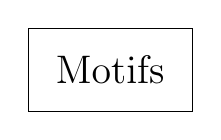
\begin{tikzpicture}
\node[draw,rectangle,inner sep=10pt] {\Large Motifs};
\end{tikzpicture}}

1) La catégorie $\mathcal{M}^+(X)$

2) Variance pour $X$

3) Cas $X=\varprojlim X_i$

4) Foncteurs $T_\ell$

5) Les $\mathbb{Q}_\ell(\unsure{+n|\pm n})$

6) La catégorie $\mathcal{M}(X)$

7) Les foncteurs $\operatorname{Hom}$ et $\operatorname{RHom}$

8) Motifs constants, tordus, et \unsure{pl. con.}

9) Filtrations de $\mathcal{M}(X)$ et $\mathcal{M}^+(X)$

10) Anneaux $\mathrm{M}^+(X)$ et $\mathrm{M}(X)$.

11) Interprétation topologique des
\deleted{\unsure{types d'isomotifs|types d'isomorphie}}\inserted{niveaux}
par la filtration canonique d'une variété proj. non singulière.

12) L'hom $L(k)\longrightarrow \mathrm{M}^+(k)$ et invariants birationnels fondamentaux.

[NB. À généraliser à des coefficients quelconques]

13) Caractérisation galoisienne des filtrations (conj. de Tate)

14) Invariants de Galois et homs de commutation.

15) Cohomologie absolue des motifs. Cas des schémas de type fini.

16) Relations avec les pts rationnels et la \unsure{cl.} des VA sur
un schéma de type fini.

17) Formes positives.

18) Motifs et fonctions $L$

19) Relations avec la cohomologie de Hodge \dots
